
\documentclass[letterpaper,hide notes,xcolor={table,svgnames},pdftex]{beamer}
\def\showexamples{t}


%\usepackage[svgnames]{xcolor}

%% Demo talk
%\documentclass[letterpaper,notes=show]{beamer}

\usecolortheme{crane}
\setbeamertemplate{navigation symbols}{}

\usetheme{MyPittsburgh}
%\usetheme{Frankfurt}

%\usepackage{tipa}

\usepackage{hyperref}
\usepackage{graphicx,xspace}
\usepackage[normalem]{ulem}

\newcommand\SF[1]{$\bigstar$\footnote{SF: #1}}



\newcounter{tmpnumSlide}
\newcounter{tmpnumNote}

% old question code
%\newcommand\question[1]{{$\bigstar$ \small \onlySlide{2}{#1}}}
% \newcommand\nquestion[1]{\ifdefined \presentationonly \textcircled{?} \fi \note{\par{\Large \textbf{?}} #1}}
% \newcommand\nanswer[1]{\note{\par{\Large \textbf{A}} #1}}


 \newcommand\mnote[1]{%
   \addtocounter{tmpnumSlide}{1}
   \ifdefined\showcues {~\tiny\fbox{\arabic{tmpnumSlide}}}\fi
   \note{\setlength{\parskip}{1ex}\addtocounter{tmpnumNote}{1}\textbf{\Large \arabic{tmpnumNote}:} {#1\par}}}

\newcommand\mmnote[1]{\note{\setlength{\parskip}{1ex}#1\par}}

%\newcommand\mnote[2][]{\ifdefined\handoutwithnotes {~\tiny\fbox{#1}}\fi
% \note{\setlength{\parskip}{1ex}\textbf{\Large #1:} #2\par}}

%\newcommand\mnote[2][]{{\tiny\fbox{#1}} \note{\setlength{\parskip}{1ex}\textbf{\Large #1:} #2\par}}

\newcommand\mquestion[2]{{~\color{red}\fbox{?}}\note{\setlength{\parskip}{1ex}\par{\Large \textbf{?}} #1} \note{\setlength{\parskip}{1ex}\par{\Large \textbf{A}} #2\par}\ifdefined \presentationonly \pause \fi}

\newcommand\blackboard[1]{%
\ifdefined   \showblackboard
  {#1}
  \else {\begin{center} \fbox{\colorbox{blue!30}{%
         \begin{minipage}{.95\linewidth}%
           \hspace{\stretch{1}} Some space intentionally left blank; done at the blackboard.%
         \end{minipage}}}\end{center}}%
         \fi%
}



%\newcommand\q{\tikz \node[thick,color=black,shape=circle]{?};}
%\newcommand\q{\ifdefined \presentationonly \textcircled{?} \fi}

\usepackage{listings}
\lstset{%
  keywordstyle=\bfseries,
  aboveskip=15pt,
  belowskip=15pt,
  captionpos=b,
  identifierstyle=\ttfamily,
  escapeinside={(*@}{@*)},
  stringstyle=\ttfamiliy,
  frame=lines,
  numbers=left, basicstyle=\scriptsize, numberstyle=\tiny, stepnumber=0, numbersep=2pt}

\usepackage{siunitx}
\newcommand\sius[1]{\num[group-separator = {,}]{#1}\si{\micro\second}}
\newcommand\sims[1]{\num[group-separator = {,}]{#1}\si{\milli\second}}
\newcommand\sins[1]{\num[group-separator = {,}]{#1}\si{\nano\second}}
\sisetup{group-separator = {,}, group-digits = true}

%% -------------------- tikz --------------------
\usepackage{tikz}
\usetikzlibrary{positioning}
\usetikzlibrary{arrows,backgrounds,automata,decorations.shapes,decorations.pathmorphing,decorations.markings,decorations.text}

\tikzstyle{place}=[circle,draw=blue!50,fill=blue!20,thick, inner sep=0pt,minimum size=6mm]
\tikzstyle{transition}=[rectangle,draw=black!50,fill=black!20,thick, inner sep=0pt,minimum size=4mm]

\tikzstyle{block}=[rectangle,draw=black, thick, inner sep=5pt]
\tikzstyle{bullet}=[circle,draw=black, fill=black, thin, inner sep=2pt]

\tikzstyle{pre}=[<-,shorten <=1pt,>=stealth',semithick]
\tikzstyle{post}=[->,shorten >=1pt,>=stealth',semithick]
\tikzstyle{bi}=[<->,shorten >=1pt,shorten <=1pt, >=stealth',semithick]

\tikzstyle{mut}=[-,>=stealth',semithick]

\tikzstyle{treereset}=[dashed,->, shorten >=1pt,>=stealth',thin]

\usepackage{ifmtarg}
\usepackage{xifthen}
\makeatletter
% new counter to now which frame it is within the sequence
\newcounter{multiframecounter}
% initialize buffer for previously used frame title
\gdef\lastframetitle{\textit{undefined}}
% new environment for a multi-frame
\newenvironment{multiframe}[1][]{%
\ifthenelse{\isempty{#1}}{%
% if no frame title was set via optional parameter,
% only increase sequence counter by 1
\addtocounter{multiframecounter}{1}%
}{%
% new frame title has been provided, thus
% reset sequence counter to 1 and buffer frame title for later use
\setcounter{multiframecounter}{1}%
\gdef\lastframetitle{#1}%
}%
% start conventional frame environment and
% automatically set frame title followed by sequence counter
\begin{frame}%
\frametitle{\lastframetitle~{\normalfont(\arabic{multiframecounter})}}%
}{%
\end{frame}%
}
\makeatother

\makeatletter
\newdimen\tu@tmpa%
\newdimen\ydiffl%
\newdimen\xdiffl%
\newcommand\ydiff[2]{%
    \coordinate (tmpnamea) at (#1);%
    \coordinate (tmpnameb) at (#2);%
    \pgfextracty{\tu@tmpa}{\pgfpointanchor{tmpnamea}{center}}%
    \pgfextracty{\ydiffl}{\pgfpointanchor{tmpnameb}{center}}%
    \advance\ydiffl by -\tu@tmpa%
}
\newcommand\xdiff[2]{%
    \coordinate (tmpnamea) at (#1);%
    \coordinate (tmpnameb) at (#2);%
    \pgfextractx{\tu@tmpa}{\pgfpointanchor{tmpnamea}{center}}%
    \pgfextractx{\xdiffl}{\pgfpointanchor{tmpnameb}{center}}%
    \advance\xdiffl by -\tu@tmpa%
}
\makeatother
\newcommand{\copyrightbox}[3][r]{%
\begin{tikzpicture}%
\node[inner sep=0pt,minimum size=2em](ciimage){#2};
\usefont{OT1}{phv}{n}{n}\fontsize{4}{4}\selectfont
\ydiff{ciimage.south}{ciimage.north}
\xdiff{ciimage.west}{ciimage.east}
\ifthenelse{\equal{#1}{r}}{%
\node[inner sep=0pt,right=1ex of ciimage.south east,anchor=north west,rotate=90]%
{\raggedleft\color{black!50}\parbox{\the\ydiffl}{\raggedright{}#3}};%
}{%
\ifthenelse{\equal{#1}{l}}{%
\node[inner sep=0pt,right=1ex of ciimage.south west,anchor=south west,rotate=90]%
{\raggedleft\color{black!50}\parbox{\the\ydiffl}{\raggedright{}#3}};%
}{%
\node[inner sep=0pt,below=1ex of ciimage.south west,anchor=north west]%
{\raggedleft\color{black!50}\parbox{\the\xdiffl}{\raggedright{}#3}};%
}
}
\end{tikzpicture}
}


%% --------------------

%\usepackage[excludeor]{everyhook}
%\PushPreHook{par}{\setbox0=\lastbox\llap{MUH}}\box0}

%\vspace*{\stretch{1}

%\setbox0=\lastbox \llap{\textbullet\enskip}\box0}

\setlength{\parskip}{\fill}

\newcommand\noskips{\setlength{\parskip}{1ex}}
\newcommand\doskips{\setlength{\parskip}{\fill}}

\newcommand\xx{\par\vspace*{\stretch{1}}\par}
\newcommand\xxs{\par\vspace*{2ex}\par}
\newcommand\tuple[1]{\langle #1 \rangle}
\newcommand\code[1]{{\sf \footnotesize #1}}
\newcommand\ex[1]{\uline{Example:} \ifdefined \presentationonly \pause \fi
  \ifdefined\showexamples#1\xspace\else{\uline{\hspace*{2cm}}}\fi}

\newcommand\ceil[1]{\lceil #1 \rceil}


\AtBeginSection[]
{
   \begin{frame}
       \frametitle{Outline}
       \tableofcontents[currentsection]
   \end{frame}
}



\pgfdeclarelayer{edgelayer}
\pgfdeclarelayer{nodelayer}
\pgfsetlayers{edgelayer,nodelayer,main}

\tikzstyle{none}=[inner sep=0pt]
\tikzstyle{rn}=[circle,fill=Red,draw=Black,line width=0.8 pt]
\tikzstyle{gn}=[circle,fill=Lime,draw=Black,line width=0.8 pt]
\tikzstyle{yn}=[circle,fill=Yellow,draw=Black,line width=0.8 pt]
\tikzstyle{empty}=[circle,fill=White,draw=Black]
\tikzstyle{bw} = [rectangle, draw, fill=blue!20, 
    text width=4em, text centered, rounded corners, minimum height=2em]
    
    \newcommand{\CcNote}[1]{% longname
	This work is licensed under the \textit{Creative Commons #1 3.0 License}.%
}
\newcommand{\CcImageBy}[1]{%
	\includegraphics[scale=#1]{creative_commons/cc_by_30.pdf}%
}
\newcommand{\CcImageSa}[1]{%
	\includegraphics[scale=#1]{creative_commons/cc_sa_30.pdf}%
}
\newcommand{\CcImageNc}[1]{%
	\includegraphics[scale=#1]{creative_commons/cc_nc_30.pdf}%
}
\newcommand{\CcGroupBySa}[2]{% zoom, gap
	\CcImageBy{#1}\hspace*{#2}\CcImageNc{#1}\hspace*{#2}\CcImageSa{#1}%
}
\newcommand{\CcLongnameByNcSa}{Attribution-NonCommercial-ShareAlike}

\newenvironment{changemargin}[1]{% 
  \begin{list}{}{% 
    \setlength{\topsep}{0pt}% 
    \setlength{\leftmargin}{#1}% 
    \setlength{\rightmargin}{1em}
    \setlength{\listparindent}{\parindent}% 
    \setlength{\itemindent}{\parindent}% 
    \setlength{\parsep}{\parskip}% 
  }% 
  \item[]}{\end{list}} 



\usepackage{alltt}

\title{Lecture 23 --- Debugging IV }

\author{Jeff Zarnett \\ \small \texttt{jzarnett@uwaterloo.ca}}
\institute{Department of Electrical and Computer Engineering \\
  University of Waterloo}
\date{\today}

\begin{document}

\begin{frame}
  \titlepage
\end{frame}

\part{Writing Debuggable Code}
\frame{\partpage}

\begin{frame}
\frametitle{Writing Debuggable Code}
\begin{changemargin}{1cm}


\begin{quote}
	\emph{Debugging is twice as hard as writing the code in the first place. Therefore, if you write the code as cleverly as possible, you are, by definition, not smart enough to debug it.} 
\end{quote}
\hfill Brian Kernighan

\end{changemargin}
\end{frame}

\begin{frame}
\frametitle{Writing Debuggable Code}
\begin{changemargin}{1cm}

Write code that is simple and easy to understand.

Syntactically clever might be shorter, but it's hard to follow.

It might make sense now, but will it in a few months?

\end{changemargin}
\end{frame}

\begin{frame}
\frametitle{Code Style}
\begin{changemargin}{1cm}

Use a consistent style for all team members.

Easier to read the source written by others.

Including something you wrote a long time ago.

\end{changemargin}
\end{frame}

\begin{frame}
\frametitle{Variable Names}
\begin{changemargin}{1cm}

Choosing good variable names takes taste, which you can develop.

If a variable has a short lifetime, like a loop variable, then a short name
is good.

Example: {\tt for (int i = 0; i < 5; i++)}

\end{changemargin}
\end{frame}

\begin{frame}
\frametitle{Variable Names}
\begin{changemargin}{1cm}

If a variable is visible to a whole class or used in a calculation, you want a more descriptive name.

Which of the following variable names is best for storing the total gross weight: \texttt{value}, \texttt{w}, \texttt{weight}, or \texttt{totalGrossWeight}? \mnote{ Typical programming style is to mash together all the words, with a capital letter at the start of each word except the first. So ``well chosen variable name'' becomes \texttt{wellChosenVariableName}.}

\end{changemargin}
\end{frame}

\begin{frame}
\frametitle{Spread Out}
\begin{changemargin}{1cm}

Don't try to squeeze too much code into one line. \mnote{Humans, studies show, read columns much better than long lines of text. That's why newspapers (you know, the kind they make out of dead trees) have columns instead of long lines.}

\begin{center}
	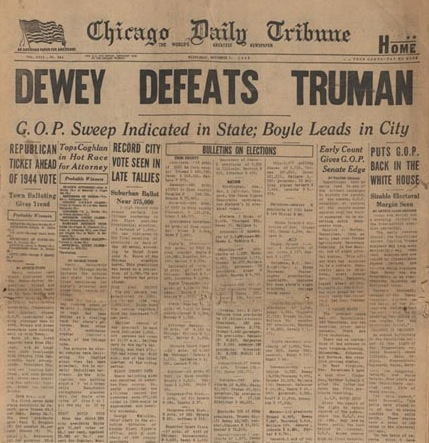
\includegraphics[width=.65\textwidth]{images/newspaper.jpg}
\end{center} 

\end{changemargin}
\end{frame}

\begin{frame}
\frametitle{Spread Out}
\begin{changemargin}{1cm}

A trivial example, but compare:\\
\texttt{if (x < 47 \&\& y > 0) \{ z = 0;\} }\\
vs.\\
\texttt{if (x < 47 \&\& y > 0) \{\\ \hspace*{0.5cm} z = 0; \\ \} }

The second is easier to read, but also easier to debug. \mnote{You can put a breakpoint now on the second line ( \texttt{z = 0;} which will trigger only when the \texttt{x} and \texttt{y} conditions are met.}

\end{changemargin}
\end{frame}

\begin{frame}
\frametitle{Use Temporary Variables}
\begin{changemargin}{1cm}
Use a temporary variable for the sub-expressions.

Instead of:\\
\texttt{return getBaseAmount() + getInsuranceCorrection() + getFreightCorrection();}\\
try:\\
\texttt{double sum = getBaseAmount() + getInsuranceCorrection() + getFreightCorrection();\\ return sum;}\\

\mnote{Once again, this makes debugging easier, because we can set a breakpoint at the creation of the sum and examine its value immediately before it is returned. If we're trying to track down an error, it's very tedious to have to enter each of the functions to see their values. It's longer, but easier to debug.}

\end{changemargin}
\end{frame}

\begin{frame}
\frametitle{Write Testable Code}
\begin{changemargin}{1cm}
Code that is testable will be easier to work with than code which is difficult to test.

If a test on a section passes, you can save time and look somewhere else first.

You might be able to adapt a unit test to help you debug:\\
\quad Invoice module is misbehaving for values above \$1~000~000 \\
\quad You have some tests which use a value like \$10~000 \mnote{Adapt these tests and see if one of them helps you identify the problem}
\end{changemargin}
\end{frame}

\begin{frame}
\frametitle{Write Testable Code: Avoid \texttt{void}}
\begin{changemargin}{1cm}
Example: minimize the use of \texttt{void} methods.

Replace the void \texttt{invoice.calculateAndAddTax();}

With: \\
\quad \texttt{Money tax = invoice.calculateTax();} \\
\quad \texttt{invoice.setTax(tax);}. 

This produces two discrete, testable methods.\\
\quad Previously there was only one harder-to-test method.


\end{changemargin}
\end{frame}

\begin{frame}
\frametitle{Write Testable Code: Performance Optimizations}
\begin{changemargin}{1cm}
Performance optimizations can be a problem.

Shortcuts and clever tricks might be faster, but harder to understand.

Use them only if they are truly necessary.

\end{changemargin}
\end{frame}


\begin{frame}
\frametitle{Comments}
\begin{changemargin}{1cm}
One view is that comments are necessary.

Another is they are dangerous: misleading when out of date.

Wrong comments are worse than no comments at all.

Write code so it's ``self-document'' (easy for an expert to understand what is going on).

\end{changemargin}
\end{frame}

\begin{frame}
\frametitle{Comment: Non-Obvious}
\begin{changemargin}{1cm}
Another view is ``comment anything non-obvious''.

Problem: obvious to one programmer is not obvious to others. \mnote{In particular, a programmer who has spent a long time looking at a module or section of code has a good understanding of what it is and how it should work. If he or she comments only what is non obvious to him/her, and then quits the company, the next person to work on this module may be faced with code that is very difficult to understand.}

Potential solution: code reviews. \mnote{A co-worker at the same company will have the basic knowledge of the software but may not know the specifics of the code under review. The reviewer can point out areas that need comments to aid in their understanding.}

\end{changemargin}
\end{frame}

\begin{frame}
\frametitle{Comments}
\begin{changemargin}{1cm}
My view: comments should be used to explain \emph{why} something is done.

Example:\\
\texttt{//We multiply the numerator and denominator by 15/16 before the division takes place}\\
vs.\\
\texttt{//We multiply the numerator and denominator by 15/16 to work around the Pentium FDIV bug}\\


\end{changemargin}
\end{frame}

\begin{frame}
\frametitle{Comments}
\begin{changemargin}{1cm}
Other things we might comment:

\begin{itemize}
	\item What the function is supposed to do.
	\item Assumptions.
	\item Parameters to a function.
	\item Bug fixes (noting the ticket number).
	\item Unexpected side effects.
	\item Workarounds (see previous slide).
\end{itemize}


\end{changemargin}
\end{frame}


\begin{frame}
\frametitle{Documentation}
\begin{changemargin}{1cm}
If the documents are crap, nobody will read them.

A small amount of good documentation is best.

Don't waste time writing too much.

Like comments, try to write self-explanatory code;\\
\quad write documents where necessary.

\end{changemargin}
\end{frame}

\begin{frame}
\frametitle{Documentation}
\begin{changemargin}{1cm}
Same problem as comments: might be out of date.

Wrong docs are worse than no docs at all.
\end{changemargin}
\end{frame}

\begin{frame}
\frametitle{Log Files}
\begin{changemargin}{1cm}
Create log files. They help in diagnosing problems.

Airplanes have ``black boxes'' that record flight data.

If there is a crash/incident, data is available to investigators.

Choose wisely how detailed the logging is.\\
\quad Too much: important data lost in the noise.\\
\quad Too little: insufficient data to reconstruct the incident.


\end{changemargin}
\end{frame}

\part{The Golden Rules of Debugging}
\frame{\partpage \mnote{We'll now sum up our section on debugging with 13 golden rules of debugging. These are some generally applicable hints that you should follow. If you are choosing to violate these rules, you'd better have a good reason.}} 

\begin{frame}
\frametitle{The Golden Rules of Debugging}
\begin{changemargin}{1cm}

Rule 1: \emph{Understand the Requirements}

Before you begin: check the specification / documentation.

Maybe the software is already doing what it is supposed to do.

\end{changemargin}
\end{frame}

\begin{frame}
\frametitle{The Golden Rules of Debugging}
\begin{changemargin}{1cm}

Rule 2: \emph{Make it Fail}

Create a test case to reproduce the failure. \mnote{This will be needed to ensure the problem is fixed when the code is changed, can be used in the regression test, and helps you understand all factors that contribute to the failure.}

Bug reports are like eyewitness accounts: incomplete, conflicting, and full of interpretation mixed with fact. \mnote{Bug reports are a bit like eyewitness accounts: they are usually incomplete, conflicting, and contain interpretation as well as fact. Even if the users are trying their best to give a truthful and complete account, it will be necessary to sort through the the data and find the facts.}

\end{changemargin}
\end{frame}

\begin{frame}
\frametitle{The Golden Rules of Debugging}
\begin{changemargin}{1cm}

Rule 3: \emph{Simplify the Test Case}

Make the test case simpler:

\begin{itemize}
	\item Rule out irrelevant factors.
	\item Reduce runtime.
	\item Make the case easier to understand.
\end{itemize}

\end{changemargin}
\end{frame}

\begin{frame}
\frametitle{The Golden Rules of Debugging}
\begin{changemargin}{1cm}

Rule 4: \emph{Look at the Right Error Message}

Which error message do we look at?

The first one!

Subsequent problems are sometimes caused by the first error.

\end{changemargin}
\end{frame}

\begin{frame}
\frametitle{The Golden Rules of Debugging}
\begin{changemargin}{1cm}

Rule 5: \emph{Check the Environment}

Check what is otherwise really obvious.\\
\quad ``Is it plugged in?'' ``Is it turned on?''\\
\quad ``Have you tried turning it off and on again?''

Is the disk full? Is there enough memory? \mnote{does the user have permissions on the operating system?}

\end{changemargin}
\end{frame}


\begin{frame}
\frametitle{The Golden Rules of Debugging}
\begin{changemargin}{1cm}

Rule 6: \emph{Separate facts from interpretation}

Examine the bug report and find out what is a fact.

Suppose the process fails on a file with a name $>32$ chars.\\
\quad Is it the file name length?\\
\quad Or the content of the file?

\end{changemargin}
\end{frame}

\begin{frame}
\frametitle{The Golden Rules of Debugging}
\begin{changemargin}{1cm}

Rule 7: \emph{Divide and Conquer}

Consider potential causes of the problem.\\
\quad Examples: Source code change, library update, OS upgrade.

Check version control history. \mnote{Start by looking at the version control history of your software. Have there been any changes to the area where things are going wrong? If one sticks out to you, you can always backtrack to just before that commit and see if the problem still occurs. If you are really stuck, go back one step at a time until you get to a version you know worked. If you find the one commit that is responsible for the bug, then you can examine the diffs of that commit to find the bug.}

If you revert all changes and the problem still happens -- check the environment.

\end{changemargin}
\end{frame}

\begin{frame}
\frametitle{The Golden Rules of Debugging}
\begin{changemargin}{1cm}

Rule 8: \emph{Use the Right Tool}

The debugger is not the only tool in your arsenal.

\begin{itemize}
	\item Memory debuggers
	\item Log files
	\item Static analysis tools
	\item Your own eyes
\end{itemize}

\end{changemargin}
\end{frame}

\begin{frame}
\frametitle{The Golden Rules of Debugging}
\begin{changemargin}{1cm}

Rule 9: \emph{Make One Change at a Time}

Make a change and test to see if it fixed it.

If it didn't, revert the change before you go on.

If you discover something else, note it for later.

\end{changemargin}
\end{frame}


\begin{frame}
\frametitle{The Golden Rules of Debugging}
\begin{changemargin}{1cm}

Rule 10: \emph{Keep an Audit Trail}

Take notes on what you have tried and the results.

Important when you work with others.

Also important to resume after an interruption.

\end{changemargin}
\end{frame}

\begin{frame}
\frametitle{The Golden Rules of Debugging}
\begin{changemargin}{1cm}

Rule 11: \emph{Get a Fresh Perspective}

If stuck, try explaining the problem to someone else.

They might have valuable input. \mnote{Their fresh perspective might help you to think of something you have not thought of before. If they are an expert, they may have an alternate theory, or just insight into how you might modify an existing one.}

Weird tip: explaining it to a rubber duck might help. \mnote{Neat tip: sometimes explaining the problem to an inanimate object (like a rubber duck) helps. The act of trying to explain the problem out loud (even to an object incapable of listening) might help you solve the problem.}

\end{changemargin}
\end{frame}

\begin{frame}
\frametitle{The Golden Rules of Debugging}
\begin{changemargin}{1cm}

Rule 12: \emph{If you didn't fix it...}

You changed something, the bug went away, but you don't know why...

Maybe you didn't fix the bug. Maybe it's hidden or occurs for different input.

\end{changemargin}
\end{frame}

\begin{frame}
\frametitle{The Golden Rules of Debugging}
\begin{changemargin}{1cm}

Rule 13: \emph{Create a Regression Test}

Bug fixed? Excellent.

Use the fix as the basis for a regression test.

\end{changemargin}
\end{frame}


\end{document}
